% Shared body of the manuscript: included by main.tex (Elsevier) and ieee.tex (IEEE).
\section{Introduction}\label{sec:intro}
\authornote{Draft. Statements about CEBC, ConfLVLM, Chan \& Darwiche, ImageNet-C, AMBER and Holm come from quotes you checked; all other citations still need your check against the PDF (entries marked UNVERIFIED in \texttt{refs.bib}).}

Vision--language models (VLMs) describe images fluently but often mention objects that are not there. This \emph{object hallucination} has been measured for years with CHAIR, which compares the objects named in a caption with an image's annotated objects \citep{rohrbach2018chair}, and with benchmarks such as POPE and AMBER \citep{li2023pope,wang2023amber}. A practical response is to check each mentioned object against an external source of visual evidence and to drop the mentions that the evidence does not support. Two recent methods make this step statistically principled. CEBC sets the evidence threshold at the $(1-\delta)$ quantile of a detector's scores on hallucinated mentions from a calibration set, so that ``only a small fraction (about $\delta$) of hallucinated mentions'' pass \citep[Sec.~3.3]{cebc}. ConfLVLM filters the claims of a VLM's response so that, with probability at least $1-\alpha$, the retained response contains no more than a tolerated amount of error \citep[Eq.~1]{conflvlm}. With a conformal choice of threshold, such filters carry finite-sample guarantees that hold without any model of the VLM or the detector \citep{vovk2005algorithmic,angelopoulos2023gentle}.

These guarantees rest on one assumption: the calibration data and the data the filter later sees are exchangeable. Deployed systems break it routinely. Images arrive blurred, compressed or noisy; the detector that supplies the evidence is upgraded or replaced; the filter is put in front of a newer VLM; the images come from a different source. The ConfLVLM authors name this as their main limitation: the framework ``assumes exchangeability of the calibration and test datasets'' and ``may not always hold in applications where distribution shifts frequently occur'' \citep[Limitations]{conflvlm}. CEBC observes reduced robustness ``under domain shift'' and recalibrates its threshold separately for each dataset \citep[Secs.~5.1--5.2]{cebc}. Robust conformal methods exist, but they need the shift to be described in advance: as an $\ell_2$ perturbation of given size at the test point \citep{gendler2022adversarially}, as an $f$-divergence ball whose radius must be at least the true divergence \citep{cauchois2024robust}, through a known or estimated likelihood ratio between the two covariate distributions \citep{tibshirani2019covariate}, or through weights fixed in advance whose coverage loss stays small only if the data are close to exchangeable in a total-variation sense \citep{barber2023beyond}. A detector swap or a new caption generator is not naturally described in any of these ways. For text-only language models, recent work shows that conformal factuality can fall below its target when the calibration claims come from a different generator \citep{chen2026conformalrag} or when the model configuration changes, and that recalibrating with a small labelled set from deployment largely closes the gap \citep{zhu2026configuration}; whether the same happens to detector-evidence filters for VLMs, and for which kinds of shift, has not been tested.

We therefore ask an empirical and a theoretical question. \emph{Which realistic shifts leave the clean guarantee of a calibrated hallucination filter intact without recalibration, which ones break it, why, and what is the cheapest repair that restores it?} We study the claim-level filter of CEBC and the image-level filter of ConfLVLM, both calibrated on clean COCO captions from LLaVA-1.5 scored by OWLv2, under four families of shift: 25 image degradations, two detector swaps, two VLM swaps and a move to AMBER's images.

Our contributions are:
\begin{enumerate}[leftmargin=*,itemsep=1pt]
  \item \textbf{A pre-registered shift audit of conformal VLM hallucination filters.} To our knowledge this is the first systematic test of detector-evidence conformal filters under image corruption, detector swap, VLM swap and domain change. Hypotheses, decision rules, shift parameters and analysis code were frozen in a public repository before any test caption or score was computed; every number in this paper is produced by that code (\cref{sec:design}).
  \item \textbf{A checkable sufficient condition, and evidence that it is far from necessary.} Adapting known one-sided and stochastic-dominance arguments for conformal prediction under shift \citep{clarkson2024split,doula2026conformal} to the scores of hallucinated claims, we note that a shift which makes those scores stochastically no larger keeps the clean guarantee (Proposition~\ref{prop:p1}). All 25 degradations preserved the claim-level target, yet the condition held in only \NHtwo{} of them; what matters is the change at the calibrated threshold (\cref{sec:res-s1}).
  \item \textbf{Changing the evidence source breaks the guarantee; a label-free recalibration repairs it.} Replacing OWLv2 with Grounding DINO raised the claim-level risk from \CleanClaim{} to \GdinoClaim{} against a target of 0.10. Recomputing the threshold on the new detector's scores for the same labelled calibration claims restored the target, without new annotation.
  \item \textbf{Changing the VLM breaks the claim-level guarantee but not the image-level one.} Thresholds calibrated on LLaVA-1.5 were violated on InternVL3-2B (\InternClaim{}), the VLM counterpart of the cross-generator failures reported for language models \citep{chen2026conformalrag}. An exploratory analysis suggests why: newer VLMs hallucinate less often, but the objects they do hallucinate are more often ones the detector partly sees.
  \item \textbf{A graphical-model explanation of why coupling claims does not help.} For an attractive Ising tree over a caption's claims we prove a root-dominance bound (Proposition~\ref{prop:p2}): a perturbation's influence on a claim through its neighbours is damped by $\tanh J$ per edge, so with the coupling we measure ($J=\Jlearned{}$) graph-based propagation cannot narrow robust posterior intervals. It combines the structure-free sensitivity bound of \citet{chan2002numbers} with the per-edge message contraction of \citet{ihler2005loopy}; what is new is the shared perturbation budget and the exact closed form it yields.
\end{enumerate}

% =====================================================================
\section{Related work}\label{sec:related}

\paragraph{Object hallucination and its measurement} CHAIR \citep{rohrbach2018chair} counts the COCO objects \citep{lin2014microsoft} that a caption mentions but the image's annotations do not contain; it is the labelling rule we use. POPE \citep{li2023pope} turns hallucination into yes/no questions, and AMBER \citep{wang2023amber} provides an LLM-free benchmark with annotated present objects and annotated ``hallucinatory target objects'' that models are likely to imagine. Detection methods use the VLM's own signals, such as uncertainty over sampled answers \citep{zhang2024vluncertainty} or attention patterns \citep{wen2026cadmp}, external grounding \citep{zohrabi2026haloprobe}, or combinations of evidence; in this journal, \citet{huang2025evidential} detect visual hallucinations in VLMs by measuring, with Dempster--Shafer theory, the degree of conflict between positive and negative evidence built from the model's high-level features. These methods produce scores; our concern is what happens to a \emph{guarantee} attached to such a score when conditions change.

\paragraph{Conformal guarantees for generated content} Split conformal prediction turns any score into a decision rule with a finite-sample guarantee under exchangeability \citep{vovk2005algorithmic,angelopoulos2023gentle}; conformal risk control extends this from coverage to expected losses \citep{angelopoulos2022conformal}. For language models, \citet{mohri2024language} remove low-confidence sub-claims until the output is correct with probability at least $1-\alpha$ under exchangeability, and \citet{cherian2024large} add group-conditional guarantees and adaptively lower the guaranteed level to keep outputs useful. For VLMs, ConfLVLM applies the same idea to claims about images \citep{conflvlm}, CEBC calibrates a detector-evidence threshold on hallucinated object mentions and combines it with candidate selection and constrained rewriting \citep{cebc}, and BCEA lets a VLM answer, abstain, or re-examine the image (zoom, crop or a claim-specific intervention) under a compute budget, with a high-probability bound on the hallucination rate among asserted claims \citep{xu2026bcea}. Their guarantees are stated for exchangeable (in BCEA's theorem, i.i.d.) calibration and test data, and CEBC, for example, recalibrates when the dataset changes \citep[Sec.~5.2]{cebc}. Under shift, \citet{chen2026conformalrag} find that conformal factuality for retrieval-augmented LLMs ``is not robust to distribution shifts'', for example when GPT-4 calibration claims are used to filter claims from smaller open-source LLMs, and that adding distractors to the calibration set raises factuality at a high cost in informativeness; \citet{zhu2026configuration} show that changing the prompt template, decoding temperature or quantization ``consistently erodes'' coverage, and that a recalibration using 50 labelled deployment examples, triggered by a label-free shift check, largely closes the undercoverage gap; and CoFact reweights calibration samples (prompt--response pairs) by online density-ratio estimation, with an exact guarantee when the true ratio is known and a time-averaged guarantee whose gap vanishes asymptotically when it is estimated \citep{hu2026cofact}. For VLMs, BCEA shows that reusing a threshold after its own evidence-acquisition step raises scores and breaks the guarantee, and recalibrates \citep{xu2026bcea}, and IntroConformal assumes calibration and test data from the same distribution, tests robustness only to label noise, and states that fine-tuning or checkpoint changes ``require recalibration'' \citep[Limitations]{atabuzzaman2026introconformal}. We take one step back and ask which realistic shifts make recalibration necessary for detector-evidence VLM filters, and which do not.

\paragraph{Conformal prediction under distribution shift} Under covariate shift with the conditional distribution of $Y$ given $X$ unchanged and a known likelihood ratio, weighting the calibration scores restores validity; an estimated ratio is supported empirically \citep{tibshirani2019covariate}. Without exchangeability, the coverage loss of (weighted) split conformal prediction is bounded by a weighted sum of total-variation distances between the data and the data with the test point swapped with each calibration point \citep[Theorem~2]{barber2023beyond}; their bound applies to standard unweighted split conformal prediction too, which is one reason why mild shifts can cost little coverage. Robust approaches guarantee coverage for every test distribution in an $f$-divergence ball \citep{cauchois2024robust} or under bounded $\ell_2$ perturbations of the input \citep{gendler2022adversarially}. These results need the form of the shift in advance and either its size, an upper bound on it, or the likelihood ratio; the robust-validation radius, for instance, must be at least the true divergence and is chosen by a heuristic from validation data \citep[Sec.~3]{cauchois2024robust}. Closest to our Proposition~\ref{prop:p1}, one-sided comparisons of score distributions characterise when transported or contaminated calibration stays valid: \citet{doula2026conformal} bound miscoverage by the one-sided gap between transported-source and target score distributions, note that the opposite deviation makes the transported calibration conservative, and test this on image classifiers under ImageNet-C-style corruptions, \citet{clarkson2024split} obtain over- or under-coverage under stochastic-dominance assumptions on contaminated calibration scores, and \citet{lee2026diagnosing} observe empirically that coverage collapses when test scores shift to the right. Our shifts are discrete changes of pipeline component (detector, VLM) or realistic corruptions \citep{hendrycks2019benchmarking}; instead of bounding them, we measure them, apply the one-sided condition to the scores of hallucinated claims, and test both the condition and the guarantee directly.

\paragraph{Sensitivity of probabilistic graphical models} How much a posterior can move when a parameter moves is a classical question for Bayesian networks. \citet{chan2002numbers} show that, for a binary variable, a change in one parameter changes the log-odds of any query by at most the parameter's own log-odds change, for any network structure, and note that specific topologies can be more robust. \citet{chan2005distance} bound the change in any conditional odds by a distance between two distributions, which for a network equals the distance between the old and new versions of the one conditional distribution that was changed, and \citet{chan2005markov} extend sensitivity analysis to Markov networks. For belief propagation, \citet{ihler2005loopy} prove that message errors contract at each update, with slope $\tanh(\log d(\psi))$ for an edge potential of dynamic range $d(\psi)$ \citep[Theorem~8]{ihler2005loopy}, which for an Ising edge is $\tanh J$, but with a separate error cap per message or potential rather than a shared budget; \citet{mooij2008bounds} propagate box bounds on marginals, and \citet{hopkins2024adversarially} study belief propagation on ferromagnetic Ising trees with zero field when an adversary flips a fraction of the observed leaves, which is a shared budget on observations rather than on the model's fields. These bounds are tight in the worst case and do not depend on where the query sits in the graph; our Proposition~\ref{prop:p2} adds structure (an attractive Ising tree), perturbs the potentials rather than the observations, couples the per-node radii through one shared budget rather than independent boxes, and uses the tree contraction to show that coupling a caption's claims cannot narrow their robust intervals at the coupling strengths we measure.

% =====================================================================
\section{Setting and filters}\label{sec:setting}

A VLM writes a caption for image $x$. Following CHAIR \citep{rohrbach2018chair} we extract the COCO object categories mentioned in the caption; each mention is a \emph{claim}. A claim is \emph{hallucinated} ($Y=1$) if its category is not among the image's ground-truth objects and \emph{supported} ($Y=0$) otherwise. An open-vocabulary detector scores each claim; we use the logit of the detector's maximum box probability for the query ``a photo of a $\langle$category$\rangle$'', so a larger score $S$ means more visual evidence that the object is present.

\paragraph{Claim-level filter (CEBC-style)} Let $S_1,\dots,S_m$ be the scores of the hallucinated claims in the calibration set and $k=\lceil (m+1)(1-\delta)\rceil$. The threshold is the $k$-th smallest score, $\hat\tau=S_{(k)}$ ($\hat\tau=+\infty$ if $k>m$), and a claim is kept iff $S>\hat\tau$. Its \emph{risk} is the probability that a hallucinated test claim is kept, $R_{\mathrm{c}}=\Pr(S>\hat\tau\mid Y=1)$. This is the threshold component of CEBC \citep[Sec.~3.3]{cebc}, which sets $\tau=\mathrm{clip}(\mathrm{Quantile}_{1-\delta}(\mathcal H),\tau_{\min},\tau_{\max})$ over the detector scores $\mathcal H$ of hallucinated calibration mentions (their Eq.~4) and argues that ``only a small fraction (about $\delta$) of hallucinated mentions'' then pass. We drop the clipping and use the finite-sample conformal index $k$, which turns ``about $\delta$'' into the guarantee below; CEBC states no formal guarantee or exchangeability assumption. We study only this filtering step, not CEBC's candidate selection and constrained rewriting \citep[Sec.~3.6]{cebc}.

\paragraph{Image-level filter (ConfLVLM-style, $\lambda=0$)} For image $j$ let $M_j$ be the largest score among its hallucinated claims ($-\infty$ if there are none). The threshold is the conformal $(1-\alpha)$ upper quantile of $M_1,\dots,M_n$ over calibration images, and the risk is the probability that a test image keeps at least one hallucinated claim, $R_{\mathrm{i}}=\Pr(M>\hat\tau)$. This is the guarantee $\Pr(L\le\lambda)\ge1-\alpha$ of \citet[Eq.~1]{conflvlm} with $L$ the indicator that a kept claim is hallucinated and tolerance $\lambda=0$; as there, an empty output (abstention) has zero loss. Our implementation differs from theirs in using CHAIR labels and detector scores instead of claims decomposed by prompting a language model and scored by internal or external confidence such as token log-probabilities or CLIP \citep[Secs.~3--4]{conflvlm}.

\paragraph{Clean guarantee} If the test claim (image) is exchangeable with the calibration claims (images), $R_{\mathrm{c}}\le\delta$ and $R_{\mathrm{i}}\le\alpha$ \citep{vovk2005algorithmic,angelopoulos2023gentle}. Both risks are \emph{unconditional false-acceptance probabilities}; neither controls the share of hallucinated claims among the claims that are kept.

\section{Theory}\label{sec:theory}

\subsection{A sufficient condition for a guarantee to survive a shift}
Under a shift, a hallucinated test claim has score $\Sh$ instead of $S$ (image level: $\Mh$ instead of $M$); the calibration data, and so $\hat\tau$, are unchanged.

\begin{proposition}[P1]\label{prop:p1}
(a) If $\Pr(\Sh>t)\le\Pr(S>t)$ for all $t\in\mathbb{R}$ (the shifted score of a hallucinated claim is stochastically no larger than its clean score), then $\Pr(\Sh>\hat\tau)\le\Pr(S>\hat\tau)\le\delta$.
(b) The same holds at image level with $M,\Mh,\alpha$.
(c) If the shift never raises the score of a hallucinated claim ($\Sh\le S$ almost surely), the conditions of (a) and (b) hold.
\end{proposition}
\begin{proof}
The test point is independent of the calibration sample and hence of $\hat\tau$. Conditioning on $\hat\tau=t$ and applying the dominance condition at that $t$,
$\Pr(\Sh>\hat\tau)=\mathbb{E}\big[\Pr(\Sh>t)|_{t=\hat\tau}\big]\le\mathbb{E}\big[\Pr(S>t)|_{t=\hat\tau}\big]=\Pr(S>\hat\tau)\le\delta$, where the last step is the clean guarantee. Part (b) is identical. For (c), $\{\Sh>t\}\subseteq\{S>t\}$ for every $t$, and $\Mh=\max_i\Sh_i\le\max_i S_i=M$.
\end{proof}

\begin{remark}
One-sided arguments of this kind are known for conformal prediction under shift and contamination \citep{doula2026conformal,clarkson2024split}; the point here is that the condition concerns only hallucinated claims and can be checked on a few labelled shifted claims. The proof uses dominance only at $t=\hat\tau$, so the condition is sufficient but far from necessary; \cref{sec:res-s1} shows that this gap matters in practice. Nothing is assumed about supported claims: a shift that lowers supported scores more than hallucinated ones keeps the risk below $\delta$ while raising the share of hallucinated claims among those kept.
\end{remark}

\subsection{Why coupling claims does not narrow robust intervals}
Model the labels $h_i\in\{-1,+1\}$ of an image's claims as an attractive Ising tree, $p(h)\propto\exp(\sum_i\theta_ih_i+\sum_{(i,j)}J_{ij}h_ih_j)$ with $J_{ij}\ge0$, so that $\Pr(h_r=+1)=\sigma(2\eta_r)$ for the effective field $\eta_r$ computed by belief propagation. Let the fields be perturbed within $|\delta_i|\le\varepsilon_i$ and $\sum_i|\delta_i|\le B$.

\begin{proposition}[P2, root dominance]\label{prop:p2}
Let\[\gamma_{\max}=\max_{i\neq r}\prod_{e\in\mathrm{path}(i\to r)}\tanh J_e<1\quad\text{and}\quad a=\min(\varepsilon_r,B).\]Then\[\eta_r+a\;\le\;\sup_\delta\eta_r(\delta)\;\le\;\eta_r+a+\gamma_{\max}(B-\varepsilon_r)_+,\]and symmetrically for the infimum. In particular, if $B\le\varepsilon_r$ the robust interval is exactly\[\big[\sigma(2(\eta_r-B)),\ \sigma(2(\eta_r+B))\big]\]and does not depend on the graph.
\end{proposition}
\begin{proof}[Proof sketch]
Root the tree at $r$. The messages into $r$ do not depend on $\delta_r$, so $\eta_r(\delta)=\eta_r(0,\delta_{-r})+\delta_r$. The lower bound is attained by $\delta=a\,e_r$. For the upper bound it suffices, by monotonicity of $\eta_r$ in each $\delta_i$ on an attractive tree, to take $\delta\ge0$. The derivative of $\eta_r$ with respect to $\delta_i$ lies in $[0,\gamma_i]$ with $\gamma_i=\prod_{e\in\mathrm{path}(i\to r)}\tanh J_e$, so by the mean value theorem $\eta_r(0,\delta_{-r})-\eta_r(0)\le\gamma_{\max}\sum_{i\ne r}\delta_i\le\gamma_{\max}(B-\delta_r)$. Hence $\eta_r(\delta)-\eta_r\le\gamma_{\max}B+(1-\gamma_{\max})\delta_r$, which is increasing in $\delta_r\le a$ and gives the bound. If $B\le\varepsilon_r$ the two bounds coincide at $a=B$, and $\eta\mapsto\sigma(2\eta)$ is increasing. The full proof is in \cref{app:p2}.
\end{proof}
In our data every claim was in the regime $B>\varepsilon_r$ (share \ShareBgtEps{}), where the graph can add at most $\gamma_{\max}(B-\varepsilon_r)\le\tanh J\,(B-\varepsilon)=\PtwoSlack{}$ to the field: coupling can only widen the interval, never narrow it below what the claim's own radius gives (\cref{sec:results}).

The ``gain $\le 1$'' ingredient is known: for a binary variable $X$ in any Bayesian network, co-varying the parameters $\theta_{x|u}$ and $\theta_{\bar x|u}=1-\theta_{x|u}$ (with $\theta_{x|u}\notin\{0,1\}$) changes the log-odds of any query $y$ given evidence $e$ by at most the change in the log-odds of $\theta_{x|u}$, ``with no assumptions whatsoever about the structure'' of the network \citep[Theorem~3.3, pp.~275--276]{chan2002numbers}. Chan and Darwiche also remark that a network with ``a specific topology'' can be more robust than this bound \citep[p.~281]{chan2002numbers}. Proposition~\ref{prop:p2} is such a case: perturbing a node's field in an attractive Ising tree is the analogue of their single-parameter change, and on a tree the gain from a non-target node is at most $\prod_e\tanh J_e<1$, which is the Ising case of the per-update contraction of \citet[Theorem~8]{ihler2005loopy}. Our addition is the analysis under one $\ell_1$ budget shared across nodes, which gives the exact interval when $B\le\varepsilon_r$.

% =====================================================================
\section{Experimental design}\label{sec:design}
The study was pre-registered: hypotheses, decision rules, shift parameters and analysis code were frozen in a public repository under the tag \texttt{prereg-v2} before any test caption or score was computed (\url{https://github.com/antonyjasfer/Budget-Coupled-Robust-Belief-Propagation-for-Visual-Hallucination-Detection}; archived at \url{https://doi.org/10.5281/zenodo.23810032}). Exploratory analyses are labelled as such.

\paragraph{Data} Calibration uses 700 clean COCO val2014 images \citep{lin2014microsoft} (\NCal{} claims), and the locked test split has 500 images (\NTest{} claims, \NTestHall{} hallucinated). The domain test uses the 804 AMBER generative images \citep{wang2023amber} not used in our pilot; claims are labelled with the \texttt{truth} (present objects, $A_{obj}$ in the paper) and \texttt{hallu} (annotated hallucinatory target objects, $H_{obj}$) lists of AMBER's annotation file, and the \NAmberUnknown{} of \NAmberClaims{} claims in neither list are excluded. This differs from AMBER's own CHAIR, which counts every vocabulary object not in $A_{obj}$ as hallucinated \citep[Eq.~2]{wang2023amber}; we keep only claims whose label was annotated, because AMBER's authors note that $H_{obj}$ is incomplete and that noun extraction can mislabel words such as ``orange'' \citep[Sec.~6]{wang2023amber}. The AMBER hallucinations we evaluate are therefore the ``likely to be imagined'' objects AMBER annotated. The 200 COCO and 200 AMBER images used in exploratory pilots are excluded by code.

\paragraph{Source pipeline} Captions from LLaVA-1.5-7B \citep{liu2024improved} (greedy decoding, prompt ``Please describe this image in detail.'', at most 512 new tokens); claims and labels with our re-implementation of CHAIR; scores from OWLv2 \citep{minderer2023scaling} (checkpoint \texttt{owlv2-base-}\allowbreak\texttt{patch16-ensemble}). Primary targets $\delta=\alpha=0.10$; 0.05 and 0.20 are secondary.

\paragraph{Shifts} (applied to test data only).
\begin{itemize}[leftmargin=*,itemsep=1pt]
  \item \textbf{S1, degradation:} four of the 15 ImageNet-C corruptions (Gaussian noise, contrast, pixelate, JPEG) and Gaussian blur, which ImageNet-C places in its extra validation set \citep[Sec.~4.1 and App.~B]{hendrycks2019benchmarking}, at five severities each. The paper does not print the severity parameters; we use those of the authors' code (\url{https://github.com/hendrycks/robustness}), re-implemented with PIL and NumPy (\cref{tab:s1params}). Gaussian noise is seeded by image and severity, so every run produces the same corrupted images.
  \item \textbf{S2, detector swap:} OWLv2 $\to$ OWL-ViT v1 \citep{minderer2022simple}; OWLv2 $\to$ Grounding DINO base \citep{liu2024grounding}. Also with the threshold recalibrated on the new detector's scores for the same calibration claims (labels do not depend on the detector).
  \item \textbf{S3, VLM swap:} LLaVA-1.5-7B $\to$ Qwen2.5-VL-3B-Instruct \citep{bai2025qwen25} and InternVL3-2B \citep{zhu2025internvl3}, same prompt, greedy, at most 512 new tokens.
  \item \textbf{S4, domain:} COCO val2014 $\to$ AMBER. AMBER's images come from the MS-COCO 2014 \emph{test} set and Unsplash \citep[App.~A.1.1]{wang2023amber}, so this is a partial domain shift (new images and annotations, a partly shared image source), not a disjoint domain.
  \item \textbf{S5, object removal (exploratory):} for one supported claim per test image, all COCO boxes of that category (enlarged by 10\%) are filled with the image's mean colour, making the claim hallucinated by construction.
\end{itemize}

\paragraph{Hypotheses} H1: every S1 condition preserves both targets (reported together with the share of supported claims kept and the abstention rate). H2: under S1, $\Sh$ is stochastically no larger than $S$. H3: at least one S2 swap violates the claim-level target. H4: recalibration repairs S2. H5: LLaVA-calibrated thresholds transfer to each S3 VLM. H6: they transfer to AMBER.

\paragraph{Estimation and decisions} Thresholds are averaged over 200 calibration resamples, each using 80\% of the calibration images. Uncertainty is quantified by an image-level cluster bootstrap with 2{,}000 resamples \citep{efron1993introduction}, since claims from one caption are not independent. A condition is \emph{violated} if the 95\% CI lies entirely above the target, \emph{preserved} if its upper bound is at most target $+\,0.03$, and \emph{inconclusive} otherwise. H2 is assessed per condition by $D^+=\max_t[\Pr(\Sh>t)-\Pr(S>t)]$ on paired hallucinated test claims and is supported if the upper bound of its 95\% CI is at most 0.03. P-values for H1 and H3--H6 are Holm-adjusted within each filter \citep{holm1979simple}.

\paragraph{Graphical model (descriptive)} A logistic unary model on the OWLv2 score and a chain Ising model over each caption's claims (in caption order) with one shared coupling $J\in[0,2]$, chosen by exact likelihood on Cal-A; inference by exact belief propagation. Robust intervals use $(\varepsilon,B)$ set to the 0.9 quantiles of the field changes caused by S1 on Cal-A.

% =====================================================================
\section{Results}\label{sec:results}

\Cref{tab:hyp} summarises the pre-registered hypotheses, \cref{fig:forest,tab:main} the non-degradation shifts and \cref{fig:s1,tab:s1} the degradations.

\begin{widetable}[t]\centering\small
\caption{Pre-registered hypotheses (target 0.10). Holm-adjusted p-values in parentheses.}\label{tab:hyp}
\resizebox{\linewidth}{!}{\begin{tabular}{@{}lp{6.2cm}ll@{}}\toprule
 & Hypothesis & Claim-level filter & Image-level filter\\\midrule
H1 & Degradation (S1) is safe & supported (0.038) & not supported (0.111) \\
H3 & A detector swap breaks the claim-level target & supported (0.000) & supported (0.000) \\
H4 & Recalibration repairs detector swaps & supported (0.011) & supported (0.002) \\
H5 & LLaVA-calibrated thresholds transfer to other VLMs & not supported (0.895) & supported (0.007) \\
H6 & Transfer to AMBER & supported (0.000) & supported (0.000) \\
H2 & $\tilde S \preceq_{st} S$ under S1 (upper CI of $D^+\le 0.03$) & \multicolumn{2}{l}{not supported (6 of 25 conditions meet the bound)} \\
\bottomrule
\end{tabular}}
\end{widetable}

\subsection{Clean reference}
On the clean test split the claim-level filter kept \CleanClaim{} of hallucinated claims and the image-level filter let \CleanImage{} of images keep a hallucination, both within the target; the claim-level filter kept \CleanKept{} of supported claims.

\subsection{Image degradation is safe, but not for the reason one might expect}\label{sec:res-s1}
All 25 degradations preserved the claim-level target (\cref{fig:s1}); risk generally \emph{fell} with severity, because degradation lowers detector evidence for all claims. At image level, three mild conditions (Gaussian noise 1, contrast 1 and 2) were inconclusive, with point estimates of 0.107--0.114 and CI upper bounds just above 0.13, so H1 was supported for the claim-level filter only. Safety came at a cost in utility: at the highest severities the claim-level filter kept as few as 21\% of supported claims and the image-level filter abstained on up to 48\% of images (\cref{fig:utility}), so a ``preserved'' guarantee alone does not certify a usable filter.

Proposition~\ref{prop:p1}'s condition held in only \NHtwo{} of 25 conditions (\cref{fig:h2}, left): mild JPEG, noise and contrast raised some hallucinated scores somewhere in the distribution. What matters for validity is the change at the calibrated threshold, which was small and mostly negative (\cref{fig:h2}, right). Where it was positive (e.g.\ Gaussian blur 1, $+0.018$) the clean filter's slack below the target absorbed it.

\begin{widefigure}[t]\centering
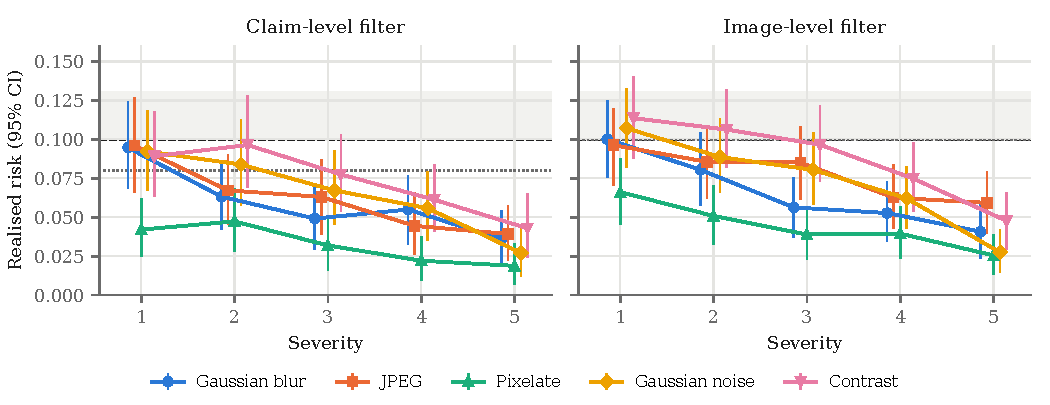
\includegraphics[width=\linewidth]{figures/fig_s1_severity.pdf}
\caption{Realised risk under image degradation (S1) for both filters, with image-level cluster-bootstrap 95\% CIs. Dashed line: target 0.10; shaded band: preservation margin (0.10--0.13); dotted line: clean risk.}\label{fig:s1}
\end{widefigure}

\begin{widefigure}[t]\centering
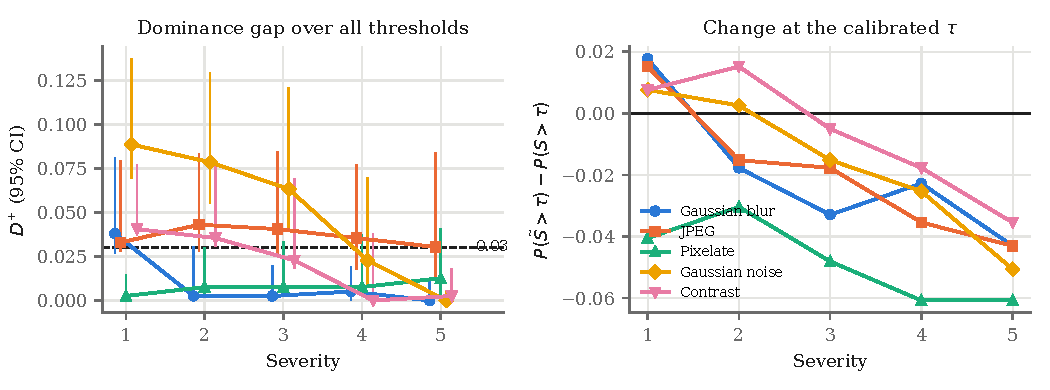
\includegraphics[width=\linewidth]{figures/fig_h2.pdf}
\caption{H2. Left: one-sided Kolmogorov--Smirnov gap $D^+$ between shifted and clean scores of hallucinated test claims (95\% CI; H2 requires the upper bound $\le0.03$). Right: the same difference evaluated only at the calibrated threshold, which is what Proposition~\ref{prop:p1} needs.}\label{fig:h2}
\end{widefigure}

\subsection{Changing the evidence source breaks the guarantee; relabelling-free recalibration repairs it}
Swapping OWLv2 for Grounding DINO broke both filters (claim level \GdinoClaim{}, image level \GdinoImage{}): Grounding DINO assigns high scores to absent objects --- its authors note that it ``will produce false positive results in some cases'' \citep[Sec.~5]{liu2024grounding} --- and its scores are not on OWLv2's scale. OWL-ViT v1, which gives hallucinated claims lower scores, made the filters conservative (\OwlvOneClaim{}). Recomputing the threshold on Grounding DINO's scores for the same labelled calibration claims restored both targets (\GdinoRecClaim{} and \GdinoRecImage{}) without any new annotation, because a claim's label does not depend on the detector.

\begin{widefigure}[t]\centering
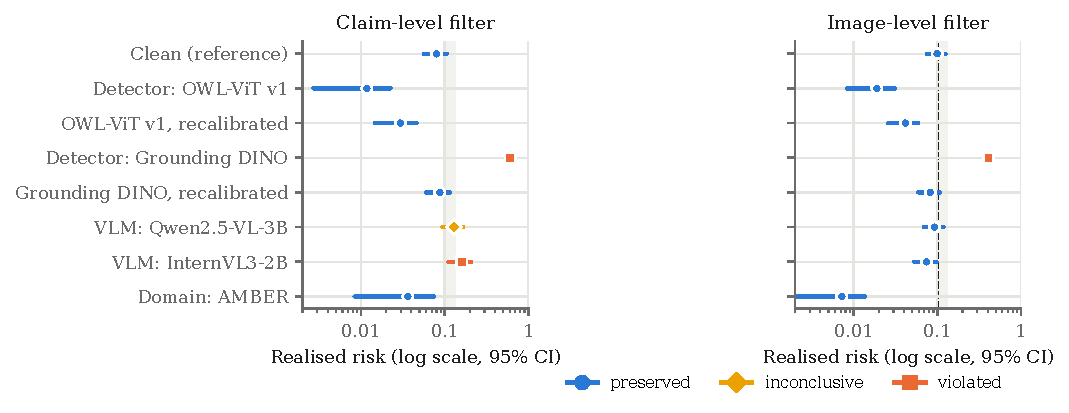
\includegraphics[width=\linewidth]{figures/fig_forest.pdf}
\caption{Realised risk (log scale, 95\% CI) for detector swaps (with and without recalibration), VLM swaps and the AMBER domain shift. Marker shape and colour give the pre-registered decision.}\label{fig:forest}
\end{widefigure}

\subsection{Changing the VLM breaks the claim-level guarantee but not the image-level one}
Thresholds calibrated on LLaVA did not transfer at claim level: InternVL3-2B was violated (\InternClaim{}) and Qwen2.5-VL-3B inconclusive (\QwenClaim{}). The image-level filter was preserved for both (\InternImage{} and \QwenImage{}). \textbf{Exploratory:} the two newer VLMs hallucinate less often (\HallRateIntern{} and \HallRateQwen{} of their claims, against \HallRateLlava{} for LLaVA; CHAIR$_i$ \ChairIntern{}, \ChairQwen{}, \ChairLlava{}), but the hallucinations they do make have a heavier upper tail of detector scores (90th percentile \HallQninetyIntern{} and \HallQninetyQwen{} against \HallQninetyLlava{} logits; \cref{fig:vlm}). The distribution of ``what gets hallucinated'' is part of what the threshold is calibrated to, and it changes with the VLM. For a user the consequence is mild: among claims kept from InternVL captions, the share that is hallucinated was \InternKeptHall{}, against \CleanKeptHall{} for LLaVA. \Cref{sec:discussion} discusses what this means for per-hallucination and per-output guarantees.

\begin{figure}[t]\centering
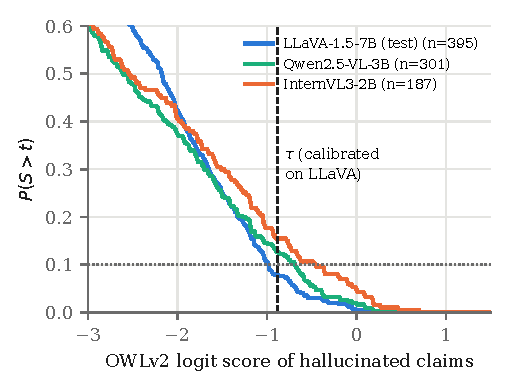
\includegraphics[width=\smallfig]{figures/fig_vlm_tails.pdf}
\caption{Exploratory. Survival function of OWLv2 scores of hallucinated claims on the test images for each VLM, with the threshold calibrated on LLaVA. The newer VLMs' hallucinations cross the threshold more often.}\label{fig:vlm}
\end{figure}

\subsection{Domain shift and object removal}
On AMBER both filters were preserved and conservative (\AmberClaim{} and \AmberImage{}). In the exploratory object-removal stress test, the clean-calibrated filters still kept the removed object's claim with probability \SfiveClaim{} (claim level) and \SfiveImage{} (image level): masking an object's boxes with the mean colour does not always remove the detector's evidence for it. A plausible but untested explanation is that the object's outline and its context outside the boxes remain visible.

\begin{widetable}[t]\centering\footnotesize\setlength{\tabcolsep}{3.5pt}
\caption{Non-degradation shifts (target 0.10). Risk [95\% CI], pre-registered decision, share of supported claims kept by the claim-level filter and abstention rate of the image-level filter.}\label{tab:main}
\resizebox{\linewidth}{!}{\begin{tabular}{@{}lllllll@{}}\toprule
Condition & Claim risk & Decision & Image risk & Decision & Kept & Abst.\\\midrule
Clean (reference) & 0.080 [0.057, 0.106] & preserved & 0.100 [0.075, 0.126] & preserved & 0.587 & 0.030 \\
Detector: OWL-ViT v1 & 0.012 [0.003, 0.023] & preserved & 0.019 [0.008, 0.031] & preserved & 0.524 & 0.103 \\
OWL-ViT v1, recalibrated & 0.030 [0.015, 0.046] & preserved & 0.041 [0.026, 0.059] & preserved & 0.606 & 0.069 \\
Detector: Grounding DINO & 0.609 [0.558, 0.657] & \textbf{violated} & 0.409 [0.365, 0.450] & \textbf{violated} & 0.970 & 0.000 \\
Grounding DINO, recalibrated & 0.087 [0.060, 0.117] & preserved & 0.083 [0.060, 0.107] & preserved & 0.599 & 0.036 \\
VLM: Qwen2.5-VL-3B & 0.129 [0.094, 0.165] & \emph{inconcl.} & 0.093 [0.070, 0.119] & preserved & 0.604 & 0.060 \\
VLM: InternVL3-2B & 0.160 [0.112, 0.208] & \textbf{violated} & 0.074 [0.053, 0.098] & preserved & 0.602 & 0.048 \\
Domain: AMBER & 0.036 [0.008, 0.074] & preserved & 0.007 [0.002, 0.014] & preserved & 0.683 & 0.152 \\
Object removed (S5, exploratory) & 0.105 [0.079, 0.132] & \emph{inconcl.} & 0.142 [0.112, 0.174] & \textbf{violated} & -- & 0.858 \\
\bottomrule
\end{tabular}}
\end{widetable}

\subsection{Graphical-model view (descriptive)}
Claim labels within a caption were almost uncorrelated (\CorrCal{} on calibration, \CorrTest{} on test data). The learned chain coupling was $J=\Jlearned{}$, so a neighbour can move a claim's field by at most $\tanh J=\TanhJ{}$ per unit of its own change; the log-likelihood gain over $J=0$ was \LLgain{} nats, and test ROC-AUC was essentially unchanged (\AucIsing{} against \AucUnary{}; \cref{tab:pgm}). Robust intervals over \RobImgs{} test images ($\varepsilon=\RobEps{}$, $B=\RobB{}$, so every claim was in the regime $B>\varepsilon_r$) were \emph{wider} with the learned coupling (mean width \WidthJ{}) than without (\WidthJzero{}), as Proposition~\ref{prop:p2} predicts: coupling gives the perturbation an extra channel and never removes the target's own.

\begin{widetable}[t]\centering\footnotesize\setlength{\tabcolsep}{3.5pt}
\caption{Classification of claims as supported (threshold 0.5 on the posterior), unary model vs.\ chain Ising model.}\label{tab:pgm}
\resizebox{\linewidth}{!}{\begin{tabular}{@{}llrrrrrrrrr@{}}\toprule
Data & Model & Acc. & Prec. & Rec. & F1 & AUC & TP & FP & TN & FN\\\midrule
Cal-A & Unary ($J=0$) & 0.820 & 0.753 & 0.502 & 0.602 & 0.859 & 128 & 42 & 641 & 127 \\
Cal-A & Chain Ising (learned $J$) & 0.823 & 0.795 & 0.471 & 0.591 & 0.861 & 120 & 31 & 652 & 135 \\
Test & Unary ($J=0$) & 0.842 & 0.784 & 0.514 & 0.621 & 0.870 & 203 & 56 & 1115 & 192 \\
Test & Chain Ising (learned $J$) & 0.836 & 0.797 & 0.468 & 0.590 & 0.871 & 185 & 47 & 1124 & 210 \\
\bottomrule
\end{tabular}}
\end{widetable}

\begin{figure}[t]\centering
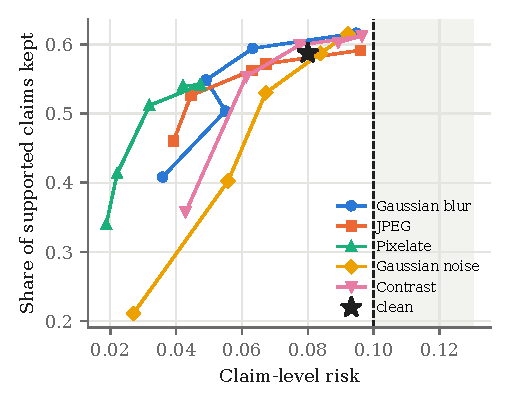
\includegraphics[width=\smallfig]{figures/fig_utility.pdf}
\caption{Utility under degradation: share of supported claims kept against claim-level risk; points along each line are severities 1--5.}\label{fig:utility}
\end{figure}

% =====================================================================
\section{Discussion}\label{sec:discussion}

\paragraph{A practical rule} For detector-evidence filters, the shifts we tested fall into two groups. Changes to the \emph{images} --- the 25 degradations and the move to AMBER --- left the clean-calibrated guarantee in place: the claim-level target was preserved in \NClaimPreservedSone{} of 25 degradations and the image-level target in \NImagePreservedSone{}, with the other three inconclusive and close to the margin. Changes to the \emph{pipeline} --- the detector that supplies the evidence and, at claim level, the VLM that writes the captions --- broke it. The rule that follows is simple: a threshold is a property of the detector's score scale and of the population of hallucinations it was calibrated on, so it must be recalibrated whenever either changes, and need not be when only the images degrade. Recalibration after a detector swap is cheap, because the labels of the calibration claims do not depend on the detector: rescoring the same claims with the new detector is enough.

\paragraph{Why degradation was benign} Degradation lowers detector evidence for every object, present or not, and so moves hallucinated claims away from the threshold. Proposition~\ref{prop:p1} formalises the safe direction, but its condition --- stochastic dominance at every threshold --- held in only \NHtwo{} of 25 conditions, while the guarantee held in all of them. Two facts explain the gap. The proof only needs dominance at the calibrated threshold, and the change at $\hat\tau$ was small or negative throughout (\cref{fig:h2}); and standard split conformal prediction degrades gracefully when the test distribution is close to the calibration distribution \citep{barber2023beyond}, so the small increases we did see were absorbed by the clean filter's slack. For practitioners this suggests checking the change at $\hat\tau$ on a few labelled shifted claims rather than testing full dominance. The other side of ``safe'' is utility: under the strongest degradation (\MinKeptSoneCond{}) the claim-level filter kept only \MinKeptSone{} of supported claims and the image-level filter abstained on \MaxAbstSone{} of images, so a preserved guarantee does not by itself make a filter useful.

\paragraph{Per-hallucination and per-output guarantees} The VLM swap separates two quantities that are easy to conflate. The claim-level risk is the probability that a \emph{hallucinated} claim is kept; it rose to \InternClaim{} on InternVL3-2B. Yet among the claims the filter kept from InternVL3-2B captions, the share that was hallucinated was \InternKeptHall{}, slightly lower than for LLaVA (\CleanKeptHall{}), and the image-level guarantee held. The newer VLM makes fewer hallucinations, but those it makes are more often objects the detector partly sees (\cref{fig:vlm}; exploratory). Which guarantee matters depends on the application: a system that must suppress a given fraction of every hallucination needs recalibration on the new VLM's claims, which requires new labels; a system that cares about how much of its output is wrong may be served by the image-level filter, which transferred. Similar cross-generator failures have been reported for language models \citep{chen2026conformalrag}; our results show that the image-level formulation can be more robust to them.

\paragraph{Graph structure does not buy robustness here} Coupling a caption's claims in an Ising chain changed accuracy and ROC-AUC very little (\cref{tab:pgm}) and made robust intervals wider, not narrower. Proposition~\ref{prop:p2} explains why: under a shared budget a perturbation is always at least as effective on the target claim as on a neighbour, whose influence is damped by $\tanh J$ per edge. With the coupling we measured ($J=\Jlearned{}$), the graph can only add an extra channel for perturbation. Coupled models could help only if claims within a caption were strongly correlated, which they were not (correlation \CorrTest{}).

\paragraph{Limitations} The audit uses one source pipeline (LLaVA-1.5-7B and OWLv2) and COCO images, plus AMBER, whose images partly come from the same COCO collection; results for other source VLMs, detectors and domains may differ. Labels come from CHAIR's synonym matching on COCO, and AMBER claims were restricted to annotated objects, so the AMBER hallucinations are those its annotators thought likely to be imagined. The swapped VLMs are small (2--3B parameters), and \TruncQwen{} of the 500 Qwen2.5-VL captions reached the 512-token limit. The object-removal stress test masks boxes with the mean colour, which leaves context and object shape partly visible. Finally, the mechanism for the VLM result is exploratory and was not pre-registered.

\section{Conclusion}
Conformal filters for VLM hallucinations carry guarantees only under exchangeability. In a pre-registered audit we found that this assumption can be relaxed for image degradation and a partial domain shift, where the clean guarantee survived, but not for changes to the pipeline: swapping the detector broke both filters until the threshold was recalibrated on the same labelled claims, and swapping the VLM broke the claim-level guarantee while the image-level one held. A simple one-sided condition explains the safe cases but is far from necessary, and a root-dominance bound shows why coupling claims in a graphical model does not make the filters more robust. Recalibrating when the evidence source or the generator changes, and checking the score change at the calibrated threshold otherwise, is a cheap way to keep these guarantees honest in deployment.

\section*{Data and code availability}
All code, the pre-registration, the frozen analysis (tag \texttt{prereg-v2}) and the scripts that produce every figure, table and number in this paper are at \url{https://github.com/antonyjasfer/Budget-Coupled-Robust-Belief-Propagation-for-Visual-Hallucination-Detection} and archived on Zenodo, \url{https://doi.org/10.5281/zenodo.23810032}. The Zenodo record contains the frozen code (tag \texttt{prereg-v2}), the scripts that build the paper, and the raw captions and detector scores (\texttt{phase4\_results.zip}, no images); code under the MIT licence, data under CC BY 4.0.

\section*{CRediT authorship contribution statement}
\todo{author list and roles, e.g. A.\ Antony Selva Jasfer: Conceptualization, Methodology, Software, Investigation, Formal analysis, Writing -- original draft.}

\section*{Declaration of competing interest}
\todo{author to confirm: The author declares no competing interests.}

\section*{Declaration of generative AI and AI-assisted technologies in the writing process}
\todo{author to confirm and edit:} During the preparation of this work the author used Claude (Anthropic) to write and test analysis code, run checks on the results, and draft and edit text. After using this tool, the author reviewed and edited the content as needed and takes full responsibility for the content of the publication.

\section*{Acknowledgements}
\todo{funding, compute (Kaggle), people who helped}

\appendix

\section{Proof of Proposition~\ref{prop:p2}}\label{app:p2}
Root the tree at $r$. For a child $c$ of $r$, belief propagation gives the message $\nu_{c\to r}=\operatorname{atanh}\big(\tanh J_{cr}\tanh\eta_{c\to r}\big)$, where $\eta_{c\to r}=\theta_c+\delta_c+\sum_{d\in\mathrm{ch}(c)}\nu_{d\to c}$ is the field of $c$ in the subtree below it, and $\eta_r=\theta_r+\delta_r+\sum_{c\in\mathrm{ch}(r)}\nu_{c\to r}$.

\emph{Step 1 (one edge).} For $f(\eta)=\operatorname{atanh}(\tanh J\tanh\eta)$ with $J\ge0$,
\[f'(\eta)=\tanh J\,\frac{1-\tanh^2\eta}{1-\tanh^2J\tanh^2\eta}\in[0,\tanh J],\]
because $0\le\tanh^2J\le1$ makes the fraction lie in $[0,1]$. This is the Ising case of the contraction of \citet[Theorem~8]{ihler2005loopy}.

\emph{Step 2 (paths).} The field $\delta_i$ of a node $i\ne r$ enters $\eta_r$ only through the messages along the unique path from $i$ to $r$. By the chain rule, $\partial\eta_r/\partial\delta_i$ is the product of the derivatives of Step~1 along that path, so $0\le\partial\eta_r/\partial\delta_i\le\gamma_i=\prod_{e\in\mathrm{path}(i\to r)}\tanh J_e$; and $\partial\eta_r/\partial\delta_r=1$. In particular $\eta_r$ is non-decreasing in every $\delta_i$.

\emph{Step 3 (budget).} By Step~2 the supremum over $\mathcal U=\{|\delta_i|\le\varepsilon_i,\ \sum_i|\delta_i|\le B\}$ is attained with $\delta\ge0$. Writing $\eta_r(\delta)=\eta_r(0,\delta_{-r})+\delta_r$ and applying the mean value theorem on the segment from $0$ to $(0,\delta_{-r})$,
\[\eta_r(\delta)-\eta_r\le\delta_r+\gamma_{\max}\sum_{i\ne r}\delta_i\le\delta_r+\gamma_{\max}(B-\delta_r)=\gamma_{\max}B+(1-\gamma_{\max})\delta_r .\]
The right side increases in $\delta_r\le a=\min(\varepsilon_r,B)$, which gives $\eta_r+a+\gamma_{\max}(B-\varepsilon_r)_+$. The lower bound is attained by $\delta=a\,e_r$. If $B\le\varepsilon_r$ the two bounds coincide, the supremum is $\eta_r+B$, and by symmetry the infimum is $\eta_r-B$. Since $\eta\mapsto\sigma(2\eta)$ is increasing, the interval for $\Pr(h_r=+1)$ is $[\sigma(2(\eta_r-B)),\sigma(2(\eta_r+B))]$. \hfill$\square$

\section{Degradation parameters and results}
\begin{table}[h]\centering\small
\caption{S1 severity parameters (severities 1--5), as in the ImageNet-C code and frozen in \texttt{src/phase4/shifts.py}.}\label{tab:s1params}
\begin{tabular}{@{}lrrrrr@{}}\toprule
Corruption & 1 & 2 & 3 & 4 & 5\\\midrule
Gaussian blur, $\sigma$ (pixels) & 1 & 2 & 3 & 4 & 6 \\
JPEG quality & 25 & 18 & 15 & 10 & 7 \\
Pixelate, resize factor & 0.6 & 0.5 & 0.4 & 0.3 & 0.25 \\
Gaussian noise, s.d.\ on $[0,1]$ & 0.08 & 0.12 & 0.18 & 0.26 & 0.38 \\
Contrast factor $c$ & 0.4 & 0.3 & 0.2 & 0.1 & 0.05 \\
\bottomrule
\end{tabular}
\end{table}
\begin{widetable}[h]\centering\scriptsize\setlength{\tabcolsep}{3pt}
\caption{All S1 conditions (target 0.10).}\label{tab:s1}
\resizebox{\linewidth}{!}{\begin{tabular}{@{}llllllll@{}}\toprule
Corruption & Sev. & Claim risk & Decision & Image risk & Decision & Kept & Abst.\\\midrule
Gaussian blur & 1 & 0.095 [0.069, 0.125] & preserved & 0.100 [0.076, 0.125] & preserved & 0.616 & 0.025 \\
 & 2 & 0.063 [0.042, 0.087] & preserved & 0.080 [0.057, 0.104] & preserved & 0.594 & 0.030 \\
 & 3 & 0.049 [0.030, 0.072] & preserved & 0.056 [0.037, 0.076] & preserved & 0.549 & 0.045 \\
 & 4 & 0.055 [0.033, 0.077] & preserved & 0.053 [0.034, 0.073] & preserved & 0.504 & 0.065 \\
 & 5 & 0.036 [0.018, 0.054] & preserved & 0.041 [0.024, 0.058] & preserved & 0.408 & 0.155 \\
\addlinespace
JPEG & 1 & 0.096 [0.066, 0.127] & preserved & 0.096 [0.070, 0.120] & preserved & 0.591 & 0.029 \\
 & 2 & 0.067 [0.046, 0.090] & preserved & 0.086 [0.062, 0.108] & preserved & 0.572 & 0.040 \\
 & 3 & 0.063 [0.039, 0.087] & preserved & 0.085 [0.062, 0.108] & preserved & 0.563 & 0.043 \\
 & 4 & 0.044 [0.026, 0.066] & preserved & 0.063 [0.043, 0.084] & preserved & 0.526 & 0.061 \\
 & 5 & 0.039 [0.022, 0.058] & preserved & 0.059 [0.040, 0.080] & preserved & 0.460 & 0.110 \\
\addlinespace
Pixelate & 1 & 0.042 [0.025, 0.062] & preserved & 0.066 [0.045, 0.088] & preserved & 0.540 & 0.048 \\
 & 2 & 0.047 [0.028, 0.068] & preserved & 0.051 [0.033, 0.070] & preserved & 0.542 & 0.050 \\
 & 3 & 0.032 [0.016, 0.049] & preserved & 0.039 [0.023, 0.055] & preserved & 0.512 & 0.072 \\
 & 4 & 0.022 [0.009, 0.037] & preserved & 0.039 [0.023, 0.057] & preserved & 0.413 & 0.153 \\
 & 5 & 0.019 [0.007, 0.033] & preserved & 0.026 [0.013, 0.039] & preserved & 0.340 & 0.258 \\
\addlinespace
Gaussian noise & 1 & 0.092 [0.067, 0.119] & preserved & 0.107 [0.082, 0.133] & \emph{inconcl.} & 0.615 & 0.035 \\
 & 2 & 0.084 [0.058, 0.113] & preserved & 0.089 [0.066, 0.113] & preserved & 0.587 & 0.044 \\
 & 3 & 0.067 [0.045, 0.093] & preserved & 0.080 [0.058, 0.105] & preserved & 0.530 & 0.079 \\
 & 4 & 0.056 [0.035, 0.079] & preserved & 0.062 [0.043, 0.083] & preserved & 0.402 & 0.181 \\
 & 5 & 0.027 [0.012, 0.045] & preserved & 0.027 [0.015, 0.042] & preserved & 0.211 & 0.480 \\
\addlinespace
Contrast & 1 & 0.089 [0.063, 0.118] & preserved & 0.114 [0.088, 0.140] & \emph{inconcl.} & 0.603 & 0.024 \\
 & 2 & 0.096 [0.069, 0.128] & preserved & 0.106 [0.082, 0.132] & \emph{inconcl.} & 0.612 & 0.023 \\
 & 3 & 0.077 [0.053, 0.103] & preserved & 0.097 [0.073, 0.122] & preserved & 0.599 & 0.026 \\
 & 4 & 0.061 [0.041, 0.084] & preserved & 0.075 [0.053, 0.098] & preserved & 0.553 & 0.060 \\
 & 5 & 0.043 [0.024, 0.066] & preserved & 0.048 [0.030, 0.066] & preserved & 0.357 & 0.262 \\
\bottomrule
\end{tabular}}
\end{widetable}

